\documentclass[a4paper]{article}
\usepackage[margin=2cm]{geometry}

\usepackage{polski}
\usepackage[utf8]{inputenc}
\usepackage[polish]{babel}
\usepackage[table]{xcolor}


\usepackage{multirow}

\usepackage{color, colortbl}


\usepackage{graphicx}

\usepackage{setspace}

\usepackage{natbib}
\definecolor{lightgray}{gray}{0.9}

\renewcommand\thesection{\arabic{section}.}
\renewcommand\thesubsection{\thesection\arabic{subsection}.}
\renewcommand\thesubsubsection{\thesubsection\arabic{subsubsection}.}
\renewcommand\theparagraph{\thesubsubsection\arabic{paragraph}.}
\renewcommand\thesubparagraph{\theparagraph\arabic{subparagraph}.}

\title{Projekt  - inżynieria E-systemów w technologii JAVA \\ Aplikacja zarządzająca wydarzeniami kulturalnymi.}
\author{\textbf{Przemysław Michalak} 181101\\ 
\textbf{Krystian Horecki} 181079 \\
\textbf{Grupa C} (śr 11.15) \\ \\ Politechnika Wrocławska}
\date{28.02.2012 r.}

\begin{document}

\maketitle
\tableofcontents


\newpage

\onehalfspace

\section{Wymagania funkcjonalne}


\subsection{Aplikacja internetowa}

\begin{table}[h!] 
\centering
\caption{Wymaganie funkcjonalne aplikacji internetowej FUN\_INT1}

\begin{tabular}{|p{2cm}|p{12cm}|} 

\hline	
	\multicolumn{2}{|>{\columncolor[gray]{.8}}c|}{Znajdowanie najbliższych wydarzeń	w sensie geograficznym}\\ \hline ID & FUN\_INT1 \\ 
	\hline \hline \multirow{2}{*}{Opis} & Użytkownik ma możliwość znalezienia wydarzeń  
	  znajdujących się najbliżej miejsca położenia podanego w aplikacji   \\	 
	\hline
	Priorytet & Wymagane \\ \hline	
	
\end{tabular}
\label{fun_int1}
\end{table}


\begin{table}[h!] 
\centering
\caption{Wymaganie funkcjonalne aplikacji internetowej FUN\_INT2}
\begin{tabular}{|p{2cm}|p{12cm}|} \hline	
	\multicolumn{2}{|>{\columncolor[gray]{.8}}c|}{Użytkownik ma możliwość dodawania wydarzeń}\\ \hline ID & FUN\_INT2 \\ \hline \hline
	 \multirow{2}{*}{Opis} &  Możliwe jest dodawanie przez użytkowników wydarzeń,   
	 które muszą być zatwierdzane przez administratora by mogły się pojawić 
	 w aplikacji, widoczne dla użytkowników \\
	 \hline Priorytet & Wymagane \\ \hline	
	
\end{tabular}
\label{fun_int2}
\end{table}

\begin{table}[h!] 
\centering
\caption{Wymaganie funkcjonalne aplikacji internetowej FUN\_INT3}
\begin{tabular}{|p{2cm}|p{12cm}|} \hline	
	\multicolumn{2}{|>{\columncolor[gray]{.8}}c|}{Przeglądanie wydarzeń}\\ \hline
	 ID & FUN\_INT3 \\ \hline \hline
	 \multirow{2}{*}{Opis} &  Aplikacja umożliwia przeglądanie wydarzeń według
	 wybranego kryterium (czas, miejsce, kategoria) \\  \hline 
	 Priorytet & Wymagane \\
	 \hline
	
\end{tabular}
\label{fun_int3}
\end{table}

\begin{table}[h!] 
\centering
\caption{Wymaganie funkcjonalne aplikacji internetowej FUN\_INT4}
\begin{tabular}{|p{2cm}|p{12cm}|} \hline	
	\multicolumn{2}{|>{\columncolor[gray]{.8}}c|}{Użytkownik ma możliwość podglądu miejsca wydarzenia}\\
	\hline ID & FUN\_INT4 \\ \hline \hline
	 \multirow{2}{*}{Opis} &  Aplikacja umożliwia uzyskanie podglądu na mapie
	 miejsca, w którym będzie odbywać się wydarzenie \\
	 \hline Priorytet & Wymagane \\
	 \hline
	
\end{tabular}
\label{fun_int4}
\end{table}

\begin{table}[h!] 
\centering
\caption{Wymaganie funkcjonalne aplikacji internetowej FUN\_INT5}
\begin{tabular}{|p{2cm}|p{12cm}|} \hline	
	\multicolumn{2}{|>{\columncolor[gray]{.8}}c|}{Aplikacja umożliwia załorzenie konta dla użytkownika}\\
	\hline ID & FUN\_INT5 \\ \hline \hline
	 \multirow{2}{*}{Opis} &  Możliwe jest założenie konta przez użytkownika,
	  oraz jego aktywacja poprzez email. \\
	  \hline Priorytet & Wymagane \\ \hline
	
\end{tabular}
\label{fun_int5}
\end{table}


\begin{table}[h!] 
\centering
\caption{Wymaganie funkcjonalne aplikacji internetowej FUN\_INT6}
\begin{tabular}{|p{2cm}|p{12cm}|} \hline	
	\multicolumn{2}{|>{\columncolor[gray]{.8}}c|}{Aplikacja umożliwia użytkownikowi dodawanie wydaerzeń do obserwowanych }\\ 
	\hline ID & FUN\_INT6 \\ \hline
	 \hline \multirow{2}{*}{Opis} &  Możliwe jest dodawanie przez użytkownika 
	 wydarzeń do ulubionych, a następnie ich podgląd na stronie konta użytkownika.
	 \\ \hline Priorytet & Wymagane
	 \\
	 \hline
	
\end{tabular}
\label{fun_int6}
\end{table}
\pagebreak
\subsection{Aplikacja mobilna}

\begin{table}[h!] 
\centering
\caption{Wymaganie funkcjonalne aplikacji mobilnej FUN\_MOB1}
\begin{tabular}{|p{2cm}|p{12cm}|} \hline	
	\multicolumn{2}{|>{\columncolor[gray]{.8}}c|}{Aplikacja umożliwia wyświetlenie wydarzeń }\\
	\hline ID & FUN\_MOB1 \\ \hline
	 \hline \multirow{2}{*}{Opis} &  Aplikacja umożliwia użytkownikowi wyświetlenie
	 wydarzeń na ekranie telefonu komórkowego. 
	 Możliwy jest określenie zakresu wyświetlania według kategorii, miejsca i
	 czasu. \\ 
	 \hline Priorytet & Wymagane
	 \\
	 \hline
	
\end{tabular}
\label{fun_mob1}
\end{table}

\begin{table}[h!] 
\centering
\caption{Wymaganie funkcjonalne aplikacji mobilnej FUN\_MOB2}
\begin{tabular}{|p{2cm}|p{12cm}|} \hline	
	\multicolumn{2}{|>{\columncolor[gray]{.8}}c|}{Aplikacja umożliwia zalogowanie się użytkownika }\\
	\hline ID & FUN\_MOB2 \\ \hline
	 \hline \multirow{2}{*}{Opis} &  Użytkownik ma możliwość zalogowania się do
	 aplikacji, co daje mu więcej funkcjonalności (dodawanie wydarzeń do
	 ulubionych). \\ \hline Priorytet & Wymagane
	 \\
	 \hline
	
\end{tabular}
\label{fun_mob2}
\end{table}

\begin{table}[h!] 
\centering
\caption{Wymaganie funkcjonalne aplikacji mobilnej FUN\_MOB3}
\begin{tabular}{|p{2cm}|p{12cm}|} \hline	
	\multicolumn{2}{|>{\columncolor[gray]{.8}}c|}{Aplikacja umożliwia dodawanie	wydarzeń do ulubionych }\\ 
	\hline ID & FUN\_MOB3 \\ \hline
	 \hline \multirow{2}{*}{Opis} & Użytkownik po zalogowaniu się, ma
	 możliwość dodawania wydarzeń do ulubionych. \\
	 \hline Priorytet & Wymagane
	 \\
	 \hline
	
\end{tabular}
\label{fun_mob3}
\end{table}


\begin{table}[h!] 
\centering
\caption{Wymaganie funkcjonalne aplikacji mobilnej FUN\_MOB4}
\begin{tabular}{|p{2cm}|p{12cm}|} \hline	
	\multicolumn{2}{|>{\columncolor[gray]{.8}}c|}{Aplikacja umożliwia poprowadzenie	użytkownika do miejsca wydarzenia}\\
	 \hline ID & FUN\_MOB4 \\ 
	\hline \hline
	 \multirow{2}{*}{Opis} &  Użytkownik po wybraniu wydarzenia ma możliwość
	 uzyskania widoku mapy, wraz z podaną trasą od miejsca aktualnego położenia
	 do miejsca w którym odbywa się wydarzenie.\\ 
	 \hline Priorytet & Wymagane
	 \\
	 \hline
	
\end{tabular}
\label{fun_mob4}
\end{table}
\pagebreak
\section{Wymagania niefunkcjonalne}
\subsection{Aplikacja internetowa}
\begin{table}[h!] 
\centering
\caption{Wymaganie niefunkcjonalne aplikacji internetowej NFUN\_INT1}
\begin{tabular}{|p{2cm}|p{12cm}|} \hline	
	\multicolumn{2}{|>{\columncolor[gray]{.8}}c|}{Aplikacja posiada przejrzysty	interfejs graficzny}\\ 
	\hline ID & NFUN\_INT1 \\ 
	\hline \hline
	 \multirow{2}{*}{Opis} &  Aplikacja dostarcza przejrzystego i prostego
	 interfejsu graficznego, o minimalistycznym charakterze \\
	 \hline
	 Priorytet & Wymagane
	 \\
	 \hline
	
\end{tabular}
\label{nfun_int1}
\end{table}

\begin{table}[h!] 
\centering
\caption{Wymaganie niefunkcjonalne aplikacji internetowej NFUN\_INT2}
\begin{tabular}{|p{2cm}|p{12cm}|} \hline	
	\multicolumn{2}{|>{\columncolor[gray]{.8}}c|}{Aplikacja posiada możliwość pobierania danych z innych serwisów}\\ 
	\hline ID & NFUN\_INT2 \\ 
	\hline \hline
	 \multirow{3}{*}{Opis} &  Aplikacja posiada możliwość pobierania danych oraz parsowania ich, w celu uzyskiwania 
	 informacji o wydarzeniach. Dane pobierane będą z grup i wydarzeń na stronie Facebook oraz strony
	 CouchSurfing. \\
	 \hline
	 Priorytet & Wymagane
	 \\
	 \hline
	
\end{tabular}
\label{nfun_int2}
\end{table}
\pagebreak
\section{Wymagania techniczne}
\subsection{Aplikacja internetowa}
\begin{table}[h!] 
\centering
\caption{Wymaganie techniczne aplikacji internetowej TECH\_INT1}
\begin{tabular}{|p{2cm}|p{12cm}|} \hline	
	\multicolumn{2}{|>{\columncolor[gray]{.8}}c|}{Język programowania}\\ 
	\hline ID & TECH\_INT1 \\ 
	\hline \hline
	 \multirow{2}{*}{Opis} & Aplikacja zostanie stworzona przy wykorzystaniu języka
	 Java EE w wersji 6 lub nowszej. \\
	 \hline
	
\end{tabular}
\label{tech_int1}
\end{table}

\begin{table}[h!] 
\centering
\caption{Wymaganie techniczne aplikacji internetowej TECH\_INT2}
\begin{tabular}{|p{2cm}|p{12cm}|} \hline	
	\multicolumn{2}{|>{\columncolor[gray]{.8}}c|}{System operacyjny}\\ 
	\hline ID & TECH\_INT2 \\ 
	\hline \hline
	 \multirow{1}{*}{Opis} & Linux \\
	 \hline
	
\end{tabular}
\label{tech_int2}
\end{table}


\subsection{Aplikacja mobilna}

\begin{table}[h!] 
\centering
\caption{Wymaganie techniczne aplikacji internetowej TECH\_MOB1}
\begin{tabular}{|p{2cm}|p{12cm}|} \hline	
	\multicolumn{2}{|>{\columncolor[gray]{.8}}c|}{Język programowania}\\ 
	\hline ID & TECH\_MOB1 \\ 
	\hline \hline
	 \multirow{2}{*}{Opis} & Aplikacja zostanie stworzona przy wykorzystaniu języka
	 Java oraz frameworka do tworzenia aplikacji na systemy Android. \\
	 \hline
	
\end{tabular}
\label{tech_mob1}
\end{table}


\begin{table}[h!] 
\centering
\caption{Wymaganie techniczne aplikacji internetowej TECH\_MOB2}
\begin{tabular}{|p{2cm}|p{12cm}|} \hline 	
	\multicolumn{2}{|>{\columncolor[gray]{.8}}c|}{Platforma}\\ 
	\hline ID & TECH\_MOB2 \\ 
	\hline \hline
	 \multirow{2}{*}{Opis} & Aplikacja zostanie stworzona na telefony posiadające system Android w wersji 2.1 lub nowszej. \\
	 \hline
	
\end{tabular}
\label{tech_mob2}
\end{table}

\end{document}





% \begin{center}
% \begin{figure}[h!]
% \fbox{
% 	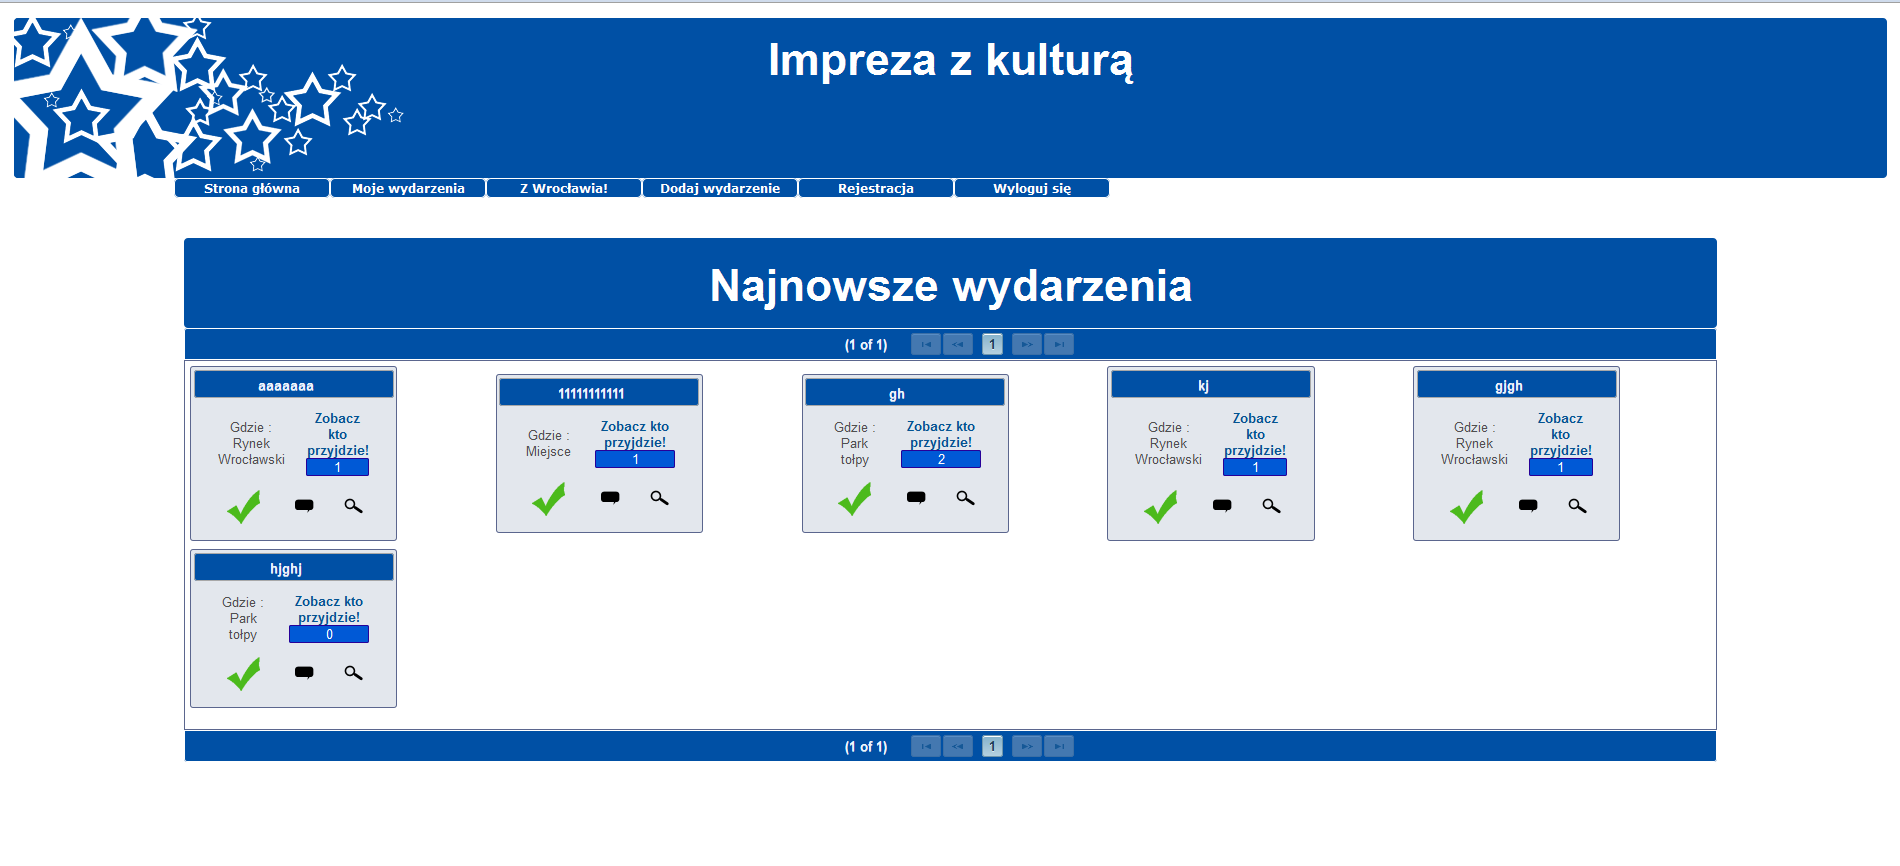
\includegraphics[width=\textwidth]{screen1.png}
% 	}
% 	\caption{Zrzut ekranu gry w momencie gdy wykryty jest tylko jeden gracz.}
% 	\label{rys1}
% \end{figure}
% \end{center}


